\documentclass[11pt]{article}
\usepackage [colon,square]{natbib}
\usepackage[mathlines]{lineno} %% <- mathlines turns on line numbering in equations
\usepackage{amsmath} 
\usepackage{printlen}
\setlength{\parindent}{10pt}
\setlength{\parskip}{10pt}
\usepackage[explicit]{titlesec}
\usepackage{helvet}
\usepackage{array}
\usepackage{printlen}
\usepackage[a4paper, margin=1.3cm]{geometry}
\usepackage{color,hyperref}
\catcode`\_=11\relax
\newcommand\email[1]{\_email #1\q_nil}
\def\_email#1@#2\q_nil{%
  \href{mailto:#1@#2}{{\emailfont #1\emailampersat #2}}
}
\newcommand\emailfont{\sffamily}
\newcommand\emailampersat{{\color{red}\small@}}
\catcode`\_=8\relax

\usepackage{hyperref}
\usepackage[export]{adjustbox}
\usepackage{bibentry}
\renewcommand{\bibfont}{\footnotesize}
\usepackage{tikz}
\usepackage{setspace}
\usepackage[inline,shortlabels]{enumitem}
\usepackage[all]{nowidow}
\def\checkmark{\tikz\fill[scale=0.4](0,.35) -- (.25,0) -- (1,.7) -- (.25,.15) -- cycle;}
\pagenumbering{gobble} 
\hypersetup{ % Remove ugly boxes around URLs
  colorlinks, linkcolor={black!100!black}, citecolor={black!50!black}, urlcolor={black!80!black}
}

\newcolumntype{L}[1]{>{\raggedright\arraybackslash}p{#1}}
\newcolumntype{C}[1]{>{\centering\arraybackslash\hspace{0pt}}p{#1}}

\linenumbers
\sloppy
\hbadness=99999 

\newcommand{\aref}[1]{\textbf{Reference #1}}
\newcommand{\TODO}[1]{\textbf{TODO: \color{red}#1}}
\newcommand{\ian}[1]{{\textbf{\color{blue}Ian says:} \color{blue} #1} }
\newcommand{\alpine}{\textit{ALPINE}\,}
\newcommand{\icesheet}{\textit{ICESHEET}\,}
\newcommand{\m}{$\,\mathrm{m}$\,}
\newcommand{\cm}{$\,\mathrm{cm}$\,}
\newcommand{\mma}{$\,\mathrm{mm  \, a^{-1}}$\,}
\newcommand{\mmma}{$\,\mathrm{m^3\, a^{-1}}$\,}
\newcommand{\mmms}{$\,\mathrm{m^3\, s^{-1}}$\,}
\newcommand{\unit}[1]{$\mathrm{#1}$}



\begin{document}
%% ------------------------------------------------------------------------ %%
% Title
% 
% (A title should be specific, informative, and brief. Use
% abbreviations only if they are defined in the abstract. Titles that
% start with general keywords then specific terms are optimized in
% searches)
% 
%% ------------------------------------------------------------------------ %%

% Example: \title{This is a test title}

\begin{center}
  \Large{\textbf{Water discharge quantity has a variable impact on sediment transport capacity in subglacial channels}}
  \normalsize

  Ian Delaney\footnote{Institut des dynamiques de la surface terrestre (IDYST), Universit\'{e} de Lausanne, B\^{a}timent G\'{e}opolis, 1015 Lausanne, Switzerland 

    ianarburua.delaney@unil.ch},
  Daniel Farinotti\footnote{Laboratory of Hydraulics, Hydrology and Glaciology (VAW), ETH-Z\"urich, H\"onggerbergring 26, 8093 89 Z\"urich, Switzerland}$^{,}$\footnote{Swiss Federal Institute for Forest, Snow and Landscape Research (WSL) Z\"uricherstrasse 111, 8903 1011 Birmensdorf, Switzerland},
  Andrew J. Tedstone\footnote{Department of Geosciences, University of Fribourg, Ch. du Musée 1700, Fribourg, Switzerland}

  

\end{center}
\paragraph{Keypoints}
\begin{itemize}
\item Water discharge variations in subglacial channels are mainly accommodated by water velocity, not channel size, given their subglacial channel's evolution.

\item Greater variability in water velocity in subglacial channels causes sediment transport capacity to vary more than in subaerial channels.

\item The channels' divergence in sediment transport response represents multiple processes represented by water discharge in sediment transport.
\end{itemize}


\begin{abstract} % 150 words
  
  \noindent
  In both subglacial and subaerial channels, the sediment transport capacity of a sediment size depends mainly on 1) the channel width over which the sediment is mobilized  and 2) water velocity, as this controls the shear stress that the flowing water applies to the channel bottom.
  In subaerial channels, changing water discharge  changes the water depth,  channel width, and velocity.
  However, in subglacial environments and on time scales of hours to weeks, changing water discharge  mainly alters the  water velocity, not channel area or width, because the subglacial conduit maintains a largely fixed geometry.
  Here, parameterizations of sediment transport capacity for pressurized flow under glaciers and subaerial open channel flow are applied to hydrographs from an Alpine glacier and the Greenland Ice Sheet.
  Results of these parameterizations show that sediment transport capacity varies far more in subglacial channels compared to subaerial channels both over time and with respect to water discharge.
  In the subglacial case, high sediment transport capacity can persist across a wide range of water discharges.
  However, changing channel width can accommodate some  variability in sediment transport capacity in subaerial channels.
  The different responses of water discharge on sediment transport capacity in subglacial channels, compared to subaerial ones, may impact the occurrence of sediment transport capacity reaching mobilization thresholds and thus should be considered in the interpretation of sediment discharge records from glaciers.


\end{abstract}

\section{Introduction}
\label{sect:intro}


Changes in glacier dynamics, geomorphology, and hydrology  have prompted numerous  recent studies of  sediment transport processes in cold regions \citep[e.g.][]{zhang2022}.
Increases in sediment transport  have been observed in Greenland \citep{bendixen2017}, the European Alps \citep{costa2017}, the Himalayas \citep{li2021}, and the Andes \citep{vergara2022}.
In some of these regions, increased water discharge and glacier melt have been interpreted to be greater sediment transport capacity \citep{bendixen2017,costa2017,li2021}.
Observed changes to sediment transport in glacierized catchments require examining the processes controlling sediment discharge in these catchments and its variations with water discharge  \citep[e.g.][]{riihimaki2005,swift2005}.

Over long periods, processes such as glacier abrasion and quarrying sculpt landscapes and create sediment to be transported fluvially from under glaciers \citep[c.f.][]{hallet1979,iverson2012,ugelvig2018}. 
On shorter time periods, pressurized water transports sediment from the under glacier \citep{walder1994,creyts2013,beaud2018}, should enough sediment be present subglacially (i.e. in a transport-limited regime).

In a transport-limited regime, sediment discharge responds to the sediment transport capacity or the amount of sediment that the water can carry.
Sediment transport capacity depends on the shear stress between water and sediment it flows  over \citep{shields1936,meyer1948,engelund1967} and the width of the channel bottom $w_c$ over which to mobilize sediment.
The shear stress  across the channel width $\tau_t$ responds to the velocity of water $v$ flowing through the channel so that 
\begin{linenomath*}
  \begin{equation}
    \label{eq:tau_t}
    \tau_t \propto w_c\, v^2,
  \end{equation}
\end{linenomath*}
% 
where $w_c$ is the width of the channel.
Following the conservation of mass, the velocity of the water flowing through a  channel is given as 
\begin{linenomath*}
  \begin{equation}
    \label{eq:v}
    v = \frac{Q_w}{S},
  \end{equation}
\end{linenomath*}
% 
where $Q_w$ is water discharge,  and $S$ is the channel's cross-sectional area.

In subaerial channels, with open channel flow, the cross-sectional area $S$ of the channel evolves with changing water discharge $Q_w$  by changing both the channel's width and the water depth \citep{leopold1953}.
During a flood with greater water discharge $Q_w$, for instance, the cross-sectional area $S$ increases as the channel widens and deepens, along with water velocity $v$, which is squared. As a result, the shear stress across the channel $\tau_t$ will increase according to Equation~\ref{eq:tau_t}. 

Yet, the response of water velocity to changing water discharge in subglacial channels differs from subaerial ones.
The size of subglacial channels responds to the creep closure of the ice above and the opening of the channel by frictional heating of water flowing through the channel \citep{rothlisberger1972}.
As a result, the subglacial channel size only evolves over days to months, whereas water discharge can vary over hours \citep[e.g.][]{iken1986,andrews2014,nanni2020}.
In turn, changes in water discharge $Q_w$ are mainly accommodated with water velocity $v$ \citep[e.g.][]{swift2005}, because the size of the channel $S$ changes on a much shorter timescale (Equation~\ref{eq:v} and Figure~\ref{fig:cartoon}).
It follows that an increase in water discharge $Q_w$ will cause the shear stress across the channel $\tau_t$ to respond to the water velocity $v$, as opposed to the subaerial channel where channel width $w_c$ evolves as well. 
\begin{center}
  \begin{figure}[h]
    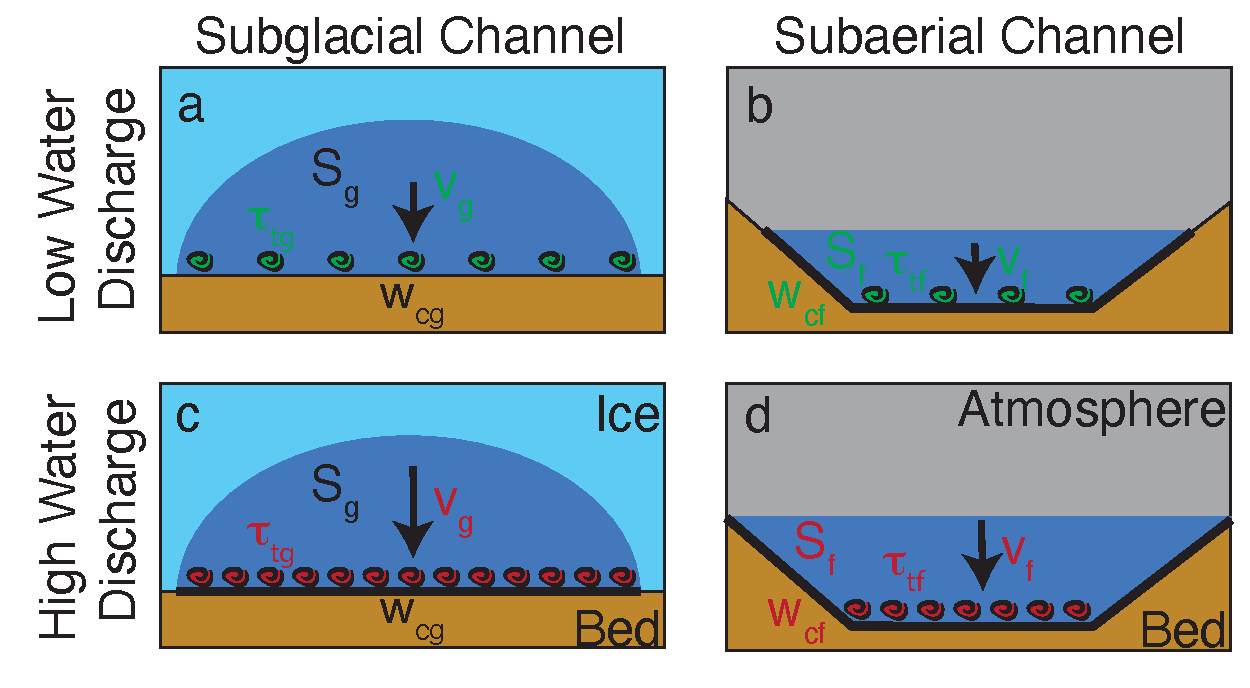
\includegraphics[width=0.8\linewidth]{Fig1.pdf}
    \caption{Sketch for the different responses that subglacial and subaerial channels have to an increase in water discharge.  Water velocity magnitude in the subglacial, $v_g$, and subaerial, $v_f$, channels are shown by arrow length. $S_g$ and $S_f$ represent the cross-sectional area in subglacial and subaerial channels. The subglacial channel widths $w_{cg}$ remain unchanged, while the subaerial channel widths evolve $w_{cf}$. Shear stress $\tau$ is responsible for the mobilization of sediment and increases with the number of makers at the channel bed. 
      Note that in the subaerial channel parameterization, channels have rectangular shapes (Section~\ref{sect:fluv}).} 
    \label{fig:cartoon}
  \end{figure}
\end{center}
% \ian{Come back to Daniel's comments}


As a result, sediment mobilization in subaerial and subglacial channels responds differently to changing water discharge.
These differences have been implicitly included in a wide range of available models that  quantify sediment transport from catchments in both subglacial and subaerial channels  \citep[e.g.][]{walder1994,tucker1997,creyts2013,wickert2019,hewitt2019}.
The divergent response of changing water discharge on sediment mobilization capacity may well impact sediment dynamics at glacier margins where flow transitions from pressurized to open channel flow \citep[e.g.][]{lane2016,perolo2018}.
Additionally, the variable response of sediment transport capacity to water discharge in the two systems may impact the interpretation of records of sediment transport in glacial systems \citep[e.g.][]{muller1968,richards2003,swift2005,ganti2016}.
Yet, the differing relationship between variations in water discharge and sediment discharge in subglacial and subaerial channels, and implications for sediment discharge records, has been minimally discussed.
Furthermore, thorough observations of water velocity and channel width in subglacial channels are limited and, to these authors' knowledge, not contrasted with subaerial conditions at the glacier margins. 

This manuscript aims to evaluate the relationship between sediment transport capacity and water discharge in subglacial channels, compared to subaerial ones.
Numerical parameterizations of subglacial and subaerial hydraulics are utilized, in the absence of observations of continuous water velocity measurements and the evolution of subglacial and subaerial channels.
Parameterizations are applied to hydrological records from an Alpine glacier in Switzerland (Fieschergletscher), and  a land-terminating glacier in Greenland (Leverett glacier).
The parameterizations' lumped and simplistic nature is intended to show the disparity between water discharge and sediment transport in subglacial systems  without considering effects such as the upstream drainage network and the role of sediment supply.
Outputs are used to explore differences in the relationships between  water discharge, channel geometry, and water velocity in the subglacial and subaerial channels. 
Furthermore, outputs are compared to sediment discharge data from these two catchments.
The manuscript then uses the demonstrated differences between the two channel types to discuss the implications for interpreting the processes driving variability in records of sediment transport from glacierized catchments.

\section{Study sites and data}
\label{sect:ss_data}

% \TODO{Address Daniel's comment: I think that these records need a few more words: where are they measured exactly? How long are the time series? What temporal resolution have they got? Do they cover the entire year, or only the summer months? }

Water and suspended sediment data are leveraged from two sites in this study.
Water discharge and suspended sediment concentration were collected at a $1$\unit{min} interval from the Fieschergletscher in the Swiss Alps  continuously over the period 2014--2021 ($46^\circ\,29'\,07"$ N, $8^\circ\,08'\,34"$ E).
A description of the data and its collection is available in \citet{felix2022} and \citet{felix2021}.

Additionally, water discharge and suspended sediment concentration were collected roughly $2$\unit{km} downstream from Leverett Glacier in Greenland over  periods from June to September from 2009 to 2012 ($67^\circ\,03'\,50"$ N, $50^\circ\,12'\,59"$ W).
This data was presented in part in \citet{cowton2012} and is available from \citet{tedstone2017} at a $5$\unit{min} time interval.
Note that in some cases the removal and relocation of sensors created variations in the sediment concentration that do not result from natural processes.

\section{Methods}
\label{sect:meth}
Parameterizations below (Sections ~\ref{sect:sub_mode}~and~\ref{sect:fluv}) represent relationships amongst water discharge, subglacial water velocity, and channel geometry in both subaerial and subglacial channels (Table \ref{table:vpm}).
Because sediment transport largely depends on shear stress applied by water flow \citep{shields1936}, both parameterizations calculate this value and integrate  it across the channel bed (Figure \ref{fig:cartoon}).
The evaluation of shear stress omits a grain size parameter and, thus, leaves open the selection of a sediment transport relationship  \citep[e.g.][]{shields1936,meyer1948} to  calculate sediment transport capacity.
As a result, relative relationships in shear stress, as opposed to sediment transport capacity, are examined.

\begin{table}[ht]
  \centering
  \caption{Variables, parameters, and constants used in this work. Where two values are given, the first refers to  \alpine{}, a case from Fieschergletscher, and the second to a glacier marginal to the \icesheet{} a case from Leverett Glacier }
  \begin{tabular}{ l  c  c c }
    Name &Symbol&  Value&Units \\ \hline
    \textbf{Variables}  & & & \\
    Water discharge  & $Q_w$& & $\mathrm{m^{3}\,s^{-1}}$ \\
    Water velocity (glacier, subaerial)  & $v_g,\,v_{f}$& & $\mathrm{m\,s^{-1}}$ \\
    Channel cross-sectional area (glacier, subaerial) &  $S_g, S_f$& & $\mathrm{m^2}$     \\
    Hydraulic diameter &$D_h$&&$\mathrm{m}$\\
    Width of channel floor (glacial, subaerial) & $w_{cg},w_{cf}$&  & $\mathrm{m}$     \\
    Hydraulic head &$\Delta h$&& $\mathrm{m}$\\
    Shear stress (glacier, subaerial) & $\tau_g,\,\tau_f$&& $\mathrm{Pa \, m^{-1}}$ \\
    Width-integrated shear stress (glacier, subaerial) & $\tau_{tg},\, \tau_{tf}$&& $\mathrm{Pa \, m^{-1}}$ \\

         &&&\\
    
    \textbf{Parameters and Constants}  & & &\\
    Gravitational constant&$g$& $9.81$&$\mathrm{m\,s^{-2}}$\\
    Density of water & $\rho_w$& $1000$ & $\mathrm{kg\,m^{-3}}$ \\
    Density of ice & $\rho_i$& $900$ & $\mathrm{kg\,m^{-3}}$ \\
    Hooke angle of channel & $\beta$ & $\frac{\pi}{2}$ & \unit{rad}\\

    Glacier thickness &$h_{ice}$& $225^a$ or $700^b$  &\unit{m}\\
    Effective glacier thickness &$h_o$&$\frac{\rho_i}{\rho_w} h_{ice}$  &\unit{m}\\
    Effective glacier length &$l$&$7000^a$ or $20,000^b$&\unit{m}\\
    Constant $1$ in Equation~\ref{eq:dS_dt} &$C_1$&$2.2\times10^{-5}$&\unit{m}$^{-1}$\\
    Constant $2$ in Equation~\ref{eq:dS_dt} &$C_2$&$3.7\times10^{-13}$&\unit{m}$^{-n}\,s^{-1}$\\
    Latent heat of fusion &$L$&$333.5 $&\unit{kJ\,kg}$^{-1}$\\
    Pressure melting coefficient &$c_t$&$7.5\times 10^{-8}$&\unit{K\,Pa}$^{-1}$\\
    Specific heat capacity of water &$c_p$&$4180$&\unit{J\,kg}$^{-1}$\unit{K}$^{-1}$\\
    
    Ice flow constant &$A$& $5.3\times10^{-24}$ &\unit{Pa}$^{-n}$\,$s^{-1}$\\
    Ice flow exponent &$n$& $3$ &$\mathrm{(-)}$\\
    Friction factor (glacier) & $f_r$ & $4$ & $\mathrm{(-)}$ \\
    Friction factor (subaerial) & $f_p$ & $3$ & $\mathrm{(-)}$\\
    Gradient of channel bed (subaerial) &$\nabla z_c$ &$0.05$& $\mathrm{(-)}$\\
    Subaerial channel factor & $k$ &$3$ & $\mathrm{s\,m^{-2}}$\\
    Channel geometry exponent &$e$& $\frac{1}{2}$&$\mathrm{(-)}$ \\
    \hline
  \end{tabular}
  \label{table:vpm}


  % $^a$ for \alpine{} (Fieschergletscher)
  
  % $^b$ for \icesheet{} (Leverett glacier)

\end{table}

\subsection{Subglacial channel  parameterization}
\label{sect:sub_mode}

To evaluate the shear stress of water flowing across sediments underneath a glacier, the subglacial channel parameterization takes into account the channel geometry and the velocity of the flowing water.
To do this, a modified version of  the lumped hydraulics model presented in \citet{clarke1996} and \citet{werder2010} is used.

Here, it is assumed that the water is transported through a subglacial channel flowing down the glacier; \citep[Figure~\ref{fig:cartoon}; ][]{rothlisberger1972}, and that the channel  size responds to frictional heating from water flow and creep closure by ice, using the Darcy-Weisbach formulation for water-flow through a pipe  \citep[e.g.][]{rothlisberger1972,clarke2003}.
The formulation here does not consider the englacial storage of water.
Thus, it is assumed that the changing hydraulic head at the top of the glacier is negligible in the evolution of the channel size. 
The evolution of subglacial channel size $S_g$ is given as
\begin{linenomath*}
  \begin{equation}
    \label{eq:dS_dt}
    \frac{\partial S_g}{\partial t} = C_1 \frac{Q \Delta h}{l} - C_2 (h_{o}-\frac{\Delta h}{2})^n\,S_g,
  \end{equation}
\end{linenomath*}
\noindent where $C_1= (1-\rho_wc_pc_t)\,\frac{\rho_wg}{\rho_iL}$ and $C_2=2A(\frac{\rho_wg}{n})^n$ are constants (Table \ref{table:vpm}), $l$ is the length of subglacial channel, $Q$ is water discharge, $\Delta h$ is the hydraulic potential change from the glacier terminus to its top, $h_{o}= \frac{\rho_i}{\rho_w} h_{ice}$ is the ice overburden pressure, and $n$ is Glen's n \citep{glen1955}.
The first term on the right side of the equation represents the opening of the channel through frictional heating, while the following term represents the creep closure of the channel from ice deformation. 


Following the Darcy-Weisbach, head drop $\Delta h$ is,
\begin{linenomath*}
  \begin{equation}
    \label{eq:dh}
    \Delta h \,  = l \,\frac{1}{g}\,s\,f_r\,\frac{Q^2}{D_h^5}
  \end{equation}
\end{linenomath*}
\noindent where $f_r$ is a friction factor, $D_h$ is the hydraulic diameter, and $l$ is the length overwhich head change occurs. $s$ is a factor accounting for channel geometry \citep{hooke1990}, calculated as:
\begin{equation}
  \label{eq:Hf}
  s = \frac{2\,(\beta -\sin \beta)^2}{(\frac{\beta}{2}\,+\,\sin \frac{\beta}{2})^4},
\end{equation}
where $\beta$ is the central angle of the circular segment that comprises the channel (the so-called Hooke angle). Note that $\beta =\pi$ corresponds to a semi-circle and
smaller values of $\beta$ result in shallow, wide channels.

With knowledge of cross-sectional area $S_g$, the shear stress, $\tau_g$, between the water and the channel bed is determined through the Darcy-Weisbach formulation
\begin{equation}
  \label{eq:tau}
  \tau_g=\frac{1}{8}\,f_r\,\rho_w\,v_g^2,
\end{equation}
% 
where  the water velocity $v_g = \frac{Q_w}{S_g}$.

The width of the flat channel floor $w_{cg}$, given angle $\beta$ is 
\begin{equation}
  \label{eq:dh2wc}
  w_{cg} = 2  \sin \frac{\beta}{2} \sqrt{\frac{2\, S_g}{\beta -\sin \beta}}.
\end{equation}

The width-integrated shear stress is represented as $\tau_{tg}=w_{cg}\,\tau_g $.

\subsection{Subaerial channel  parameterization}
\label{sect:fluv}

To parameterize the shear stress of water flowing across sediments in the subaerial channel,  the hydraulics parameterization presented in \citet{tucker1997} is implemented.
Here, given  that mass is conserved mass, there is a sufficiently wide channel so that the hydraulic radius is consistent with flow depth, and the Darcy-Weisbach relationship,
the shear stress $\tau_f$ at the river bed is represented as
\begin{linenomath*}
  \begin{equation}
    \label{eq:DW_tau}
    \tau_f=\frac{\rho_w\,g^{\frac{2}{3}}\,f_p^{\frac{1}{3}}}{2}\, \Big(\frac{Q_w}{w_{cf}} \Big)^{\frac{2}{3}} \,\nabla z_c^{\frac{2}{3}},
  \end{equation}
\end{linenomath*}
where $\nabla z_c$ is the channel slope, and $f_p$ is the friction factor for subaerial channels.
Channel width $w_{cf}$ is 
\begin{equation}
  \label{eq:wcf}
  w_{cf} = k \, Q_w^\frac{1}{2},
\end{equation}
% 
where $k$ is a constant and the exponent is commonly given as $\frac{1}{2}$ \citep{leopold1953}.
Water velocity, $v_f$, is given by rearranging Equation \ref{eq:tau} as
\begin{equation}
  \label{eq:vf}
  v_f = \sqrt{\frac{8\,\tau_f}{f_p\,\rho_w}}.
\end{equation}
% 
As in Section~\ref{sect:sub_mode}, the width-integrated shear stress is $\tau_{tf}=w_{cf}\,\tau_f$.

\subsection{Implementation}
\label{sect:imp}

The parameterizations above are applied to hydrological records from the Fieschergletscher in the Swiss Alps and the Leverett glacier on the Greenland Ice Sheet.
The hydrographs applied to the subglacial and subaerial parameterizations represent the subglacial flow of water as it leaves the glacier and transitions to subaerial flow in front of the glacier, as water moves through the catchment.
Outputs of the parameterizations are meant to represent generalizable sediment transport characteristics from these hydrographs, rather than actual hydraulic conditions.
To generalize these cases, the Fieschergletscher case is referred to as \alpine{} and is exemplified by relatively thin ice thickness ($h_{ice}$: $225$\,\unit{m}), low water discharge ( $\le\,20$\unit{m}$^3$\,\unit{s}$^{-1}$) and high diurnal variability in water discharge (Figure~\ref{fig:model_outs}, a).
The Leverett glacier case is referred to as \icesheet{} and is exemplified by thick ice  ($h_{ice}$: $700$\,\unit{m}), high water discharge ($\le\,300$\unit{m}$^3$\,\unit{s}$^{-1}$)  and low diurnal variability in water discharge (Figure~\ref{fig:model_outs}, e).

The parameterizations are first applied to a reference test case for each glacier that assumes  subglacial channel with $\beta=\frac{\pi}{2}$ and friction factors $f_r$ and $f_p$ are tuned so that the model reproduces reasonable velocities for both  the Greenland Ice Sheet and Alpine glaciers \citep[$\sim\,1.6\,$\unit{m}$^3$\,\unit{s}$^{-1}$][]{werder2010b,chandler2013}.
In both subaerial channels, the bed slope, $\nabla z_c$ is $0.05$.
Water velocity, shear stress, and width-integrated shear stress in the subglacial and subaerial channels from this formulation are presented below.  

Second, to characterize the variability in sediment discharge capacity in subglacial compared to subaerial channels further, $100$  parameterizations are applied to a range of different channel geometry factors ($\beta$ and $k$) and friction factors ($f_r$ and $f_p$).
Model runs with parameter combinations  are culled if their mean subglacial water velocity over the season lies outside of the range between $0.75$\,\unit{m}$^3$\,\unit{s}$^{-1}$ and $2$\,\unit{m}$^3$\,\unit{s}$^{-1}$ or if subaerial water velocity lies outside of the range $0.3$\,\unit{m}$^3$\,\unit{s}$^{-1}$ and $1.2$\,\unit{m}$^3$\,\unit{s}$^{-1}$, in accordance with some measurements \citep[e.g.]{werder2010b,magnusson2012,chandler2013}.
The standard deviation of a model output over the course of the season is used to quantify the variability of the model output.

Lastly, model outputs are compared with the record of sediment discharge from the two glaciers using Spearman rank correlation to reduce the impact of the non-linear response of sediment discharge to the output.

\section{Results}

\subsection{Role of water discharge in sediment transport capacity}
\begin{figure}[h]
  \centering
  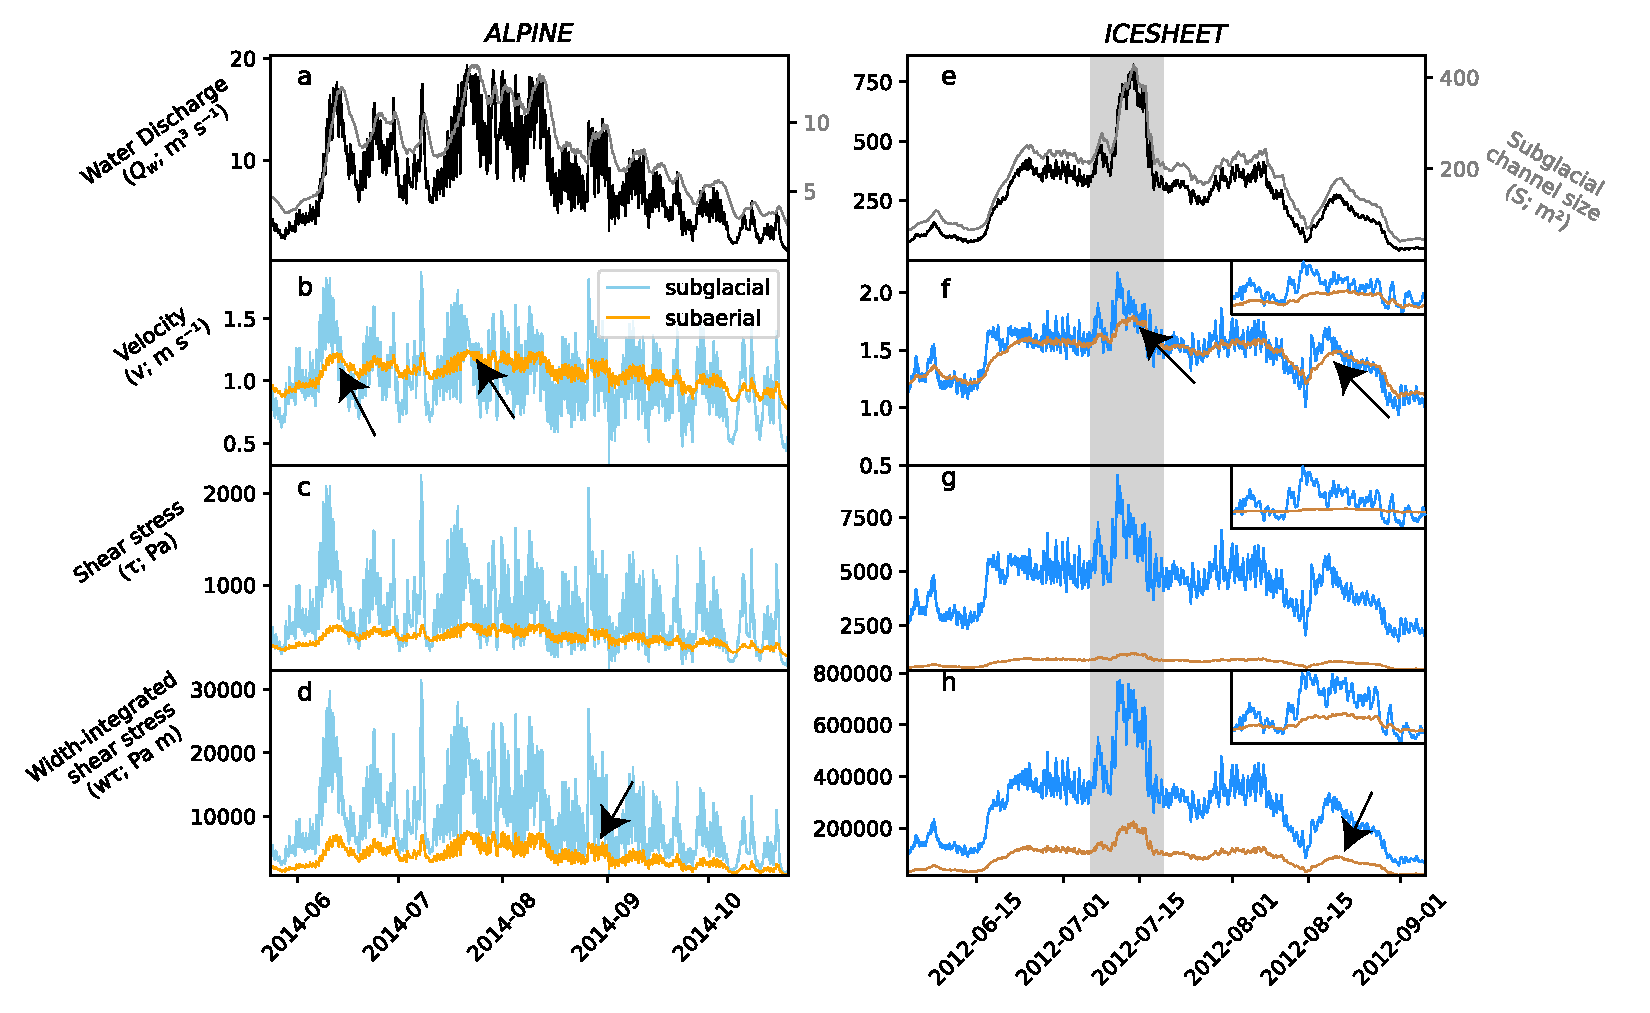
\includegraphics[width=0.9\linewidth]{Fig2.pdf}
  \caption{Model outputs resulting from the hydrographs shown in panels a and e for the cases called \alpine (a-d) and \icesheet{} (e-h).". Gray (black) lines in a and e represent the subglacial channel size (water discharge).  In other panels, blue lines represent model outputs from the subglacial channel, while orange lines represent the subaerial channel.
    Data in plots are at $15$\unit{min} intervals.
    Arrows denote some events where the variable peaks in the subglacial channel prior to the subaerial one.
    Insets in e-h show the  peak melt event \icesheet{} denoted by the shaded area.
    Note that the x and y axis are different for \alpine{} and \icesheet{} such that they each cover a summer.} 
  \label{fig:model_outs}
\end{figure}
Following the parameterizations defined in Sections~\ref{sect:sub_mode}~and~\ref{sect:fluv}, the water velocity, shear stress, and width-integrated shear stress exhibit different seasonal evolutions and peaks. Water velocity and shear stress represent the potential for sediment mobilization, and width-integrated shear stress represents the total sediment transport capacity across the channel bed (Figure~\ref{fig:model_outs}).

Over the course of the season, large peaks in water velocity and shear stress, along with width-integrated shear stress, occur in response to increases in water discharge in both cases.
In the subglacial channel, these peaks generally occur over the period when water discharge increases at the fastest rate (Figure~\ref{fig:model_outs}).
Conversely, in the subaerial channel, peaks in these variables occur when water discharge is at its highest value.
As a result, peaks in the subglacial sediment transport variables occur  when water discharge change is greatest, as opposed to when the maximum amount of water discharge occurs.
The timing of the greatest rate of change in water discharge occurs before the peaks in water discharge. 
Here, sediment could be deposited in the proglacial area as the water depressurizes and is remobilized when sediment transport capacity peaks in the subaerial system.

\begin{figure}[h]
  \centering
  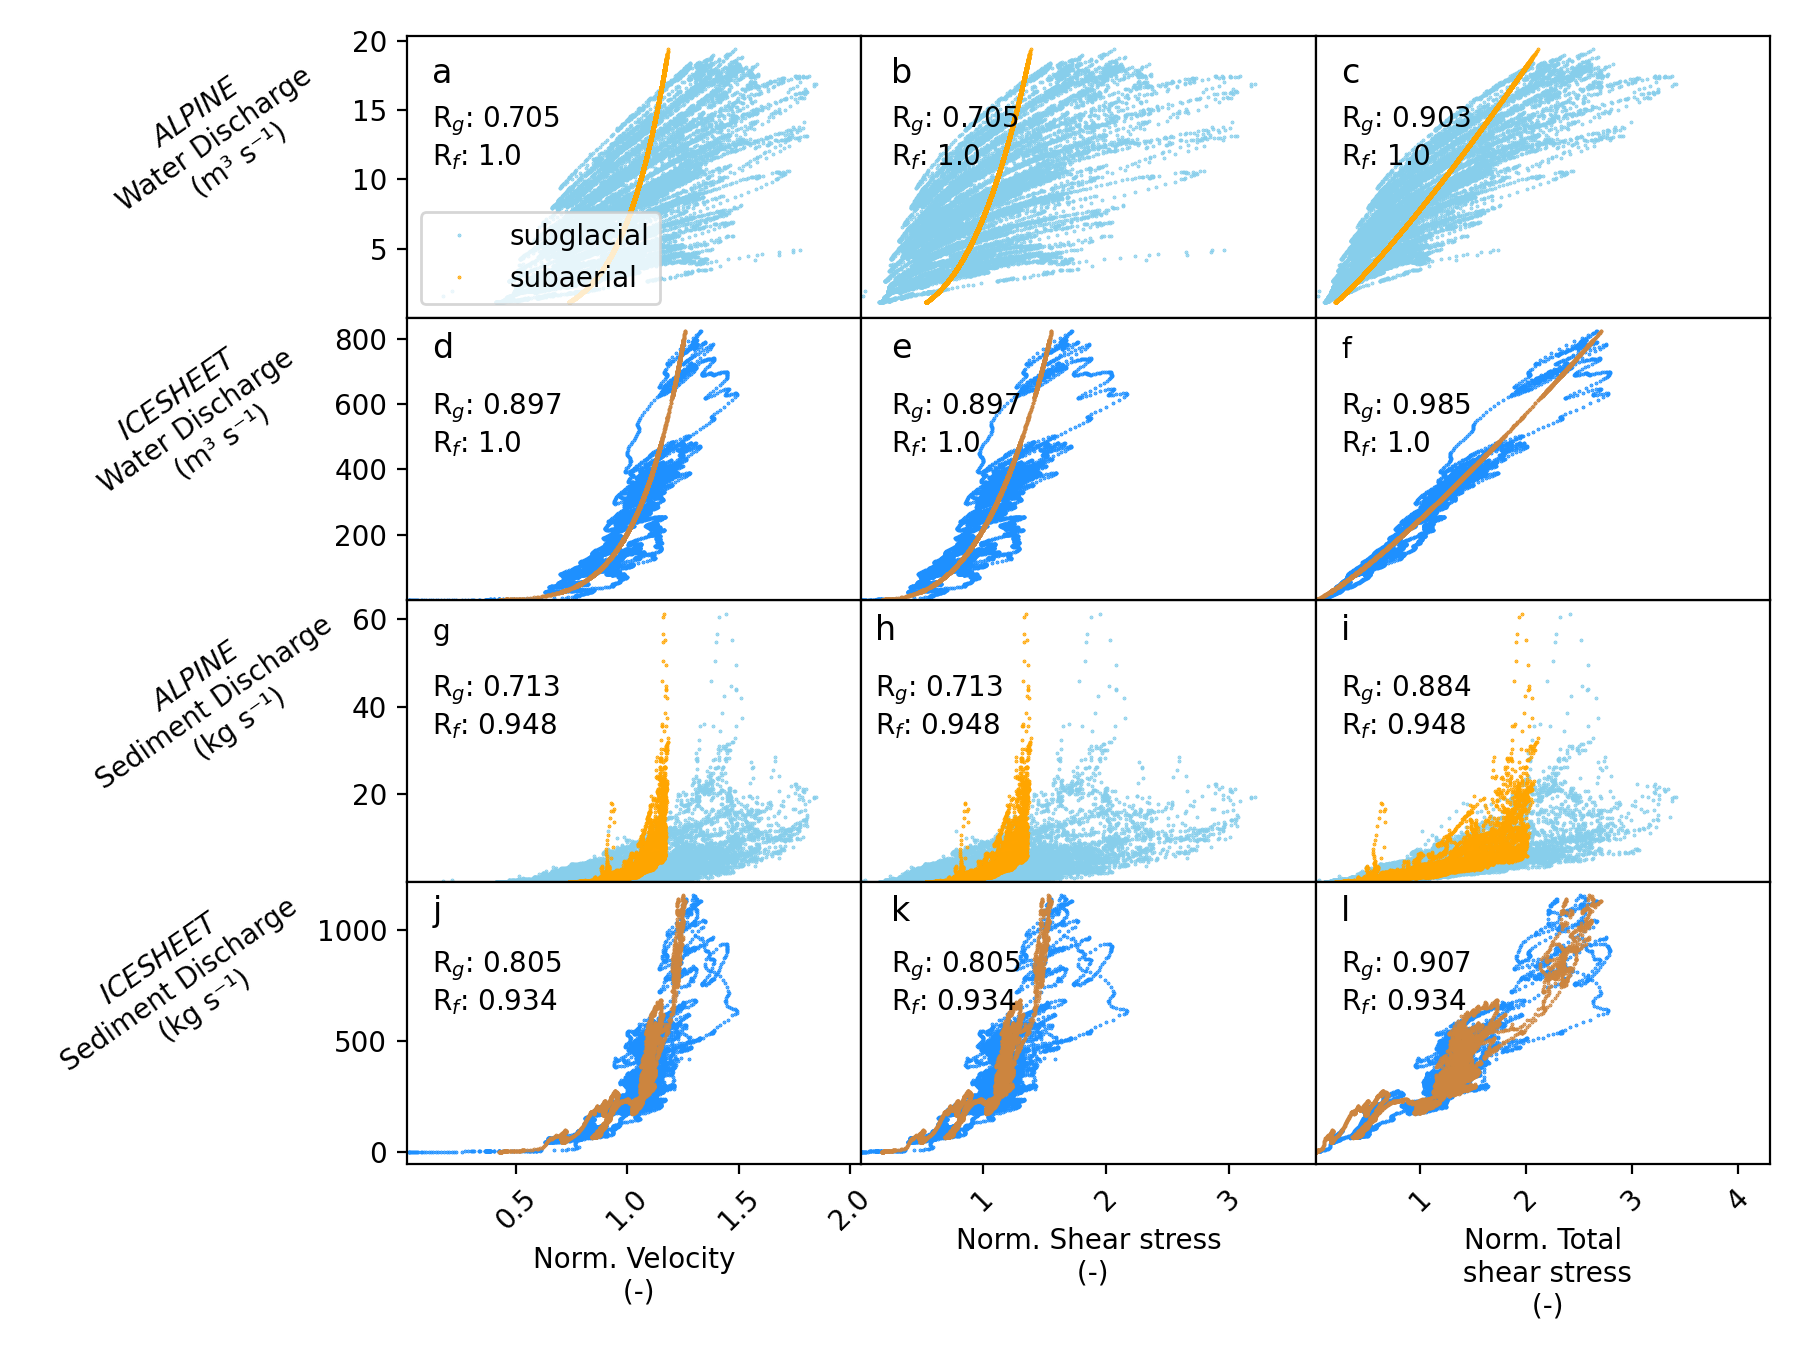
\includegraphics[width=0.9\linewidth]{Fig3.png}
  \caption{Relationship between water discharge and velocity, shear stress, and width-integrated shear stress for \alpine{}  (a-c) and \icesheet (d-f). Variables have been normalized to mean values for better comparison amongst the model runs.
    $R_g$ ($R_f$) show the Spearman rank correlation values for the subglacial (subaerial) model outputs.
    Plots are shown at $15$\unit{min} interval.} 
  \label{fig:Qw_vari}
\end{figure}

Each water discharge value in the subaerial channel is associated with a single water velocity, shear stress, and width-integrated shear stress, resulting in a perfect rank correlation between water discharge and the model output (Figure~\ref{fig:Qw_vari} a--f).
Conversely in the subglacial channel,  water velocity, shear stress, and width-integrated shear stress can vary substantially for a given water discharge and width-integrated shear stress varies with respect to the other two model outputs as well (Figure~\ref{fig:Qw_vari} a--f).
For instance, very high values of water velocity and shear stress can occur from minimal water discharge at $2.5$\,\unit{m}$^3$\,\unit{s}$^{-1}$ to the maximum water discharge at over $17$ \,\unit{m}$^3$\,\unit{s}$^{-1}$.
In \icesheet, mean values of water velocity can occur at water discharges between roughly $150$ \,\unit{m}$^3$\,\unit{s}$^{-1}$ and $310$ \,\unit{m}$^3$\,\unit{s}$^{-1}$, effectively spanning the much of the water discharge range.

When accounting for the evolving channel width of the subglacial conduit, width-integrated shear stress  across the channel generally increases with water discharge, with improved rank correlation compared to water discharge and water velocity or shear stress (Figure~\ref{fig:Qw_vari} a--f).
Yet even the width-integrated shear stress  can vary substantially, with the highest values occurring at water discharge values ranging from roughly $11$ \,\unit{m}$^3$\,\unit{s}$^{-1}$, to over $17$ \,\unit{m}$^3$\,\unit{s}$^{-1}$.
The variability in width-integrated shear stress is less pronounced in the \icesheet case, in part due to the reduced variability in water discharge.
Yet, a range of width-integrated shear stress can occur at a given discharge (Figure~\ref{fig:Qw_vari} c, f).


\begin{figure}[h]
  \centering
    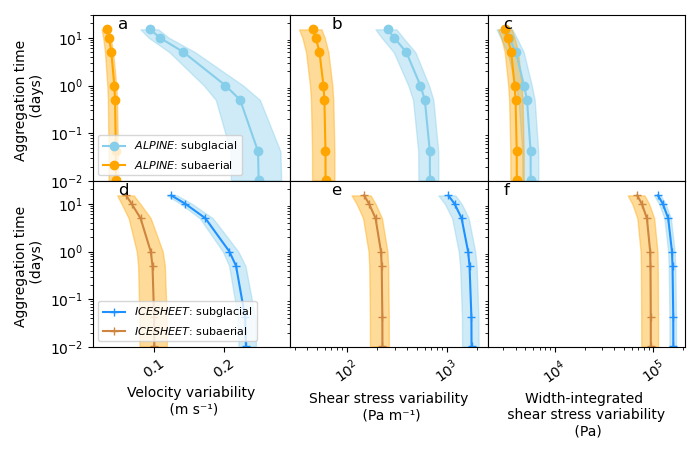
\includegraphics[width=0.9\linewidth]{Fig4.png}
    \caption{Variance (measured by the standard deviation) in water velocity, shear stress, and total shear stress for different time aggregations across a large number of subglacial and subaerial channel shapes and friction factors The subglacial (blue) and subaerial (orange) systems are distinguished as are \alpine{} (a-c) and \icesheet{} (d-f).
      Shaded areas denote the $25^{\mathrm{th}}$ and $75^{\mathrm{th}}$ quantiles of the $100$ parameter combinations tested for each of the systems (Section~\ref{sect:imp}).
      Solid lines denote  mean values.
      Time intervals shown with markers denote $15$\,\unit{min}, $1$\,\unit{hr}, $12$\,\unit{hr}, $1$\,\unit{d}, $5$\,\unit{d}, $10$\,\unit{d}, and $15$\,\unit{d} aggregation periods.
    } 
    \label{fig:multi_run}
  \end{figure}

The second model application examines the impact of a variety of channel shapes and friction factors on the relationship between water discharge and sediment transport capacity, in both systems.
Across the range of parameter values examined, variability in water velocity and shear stress remains higher in the subglacial system compared to the subaerial one.
However, in \alpine{}, the width-integrated shear stress makes the variability between the two systems comparable (Figure~\ref{fig:multi_run}).
Conversely, in \icesheet{}, with lower water discharge variability, the variability in width-integrated shear stress remains higher in the subglacial system across the time aggregation periods.

It is prescient to evaluate the time scales over which the subglacial channels may respond to changing water discharge to understand the impact on variability in sediment transport capacity.
In both cases, the variability in velocity, shear stress, and width-integrated shear stress decrease after $1-5$ day aggregations (Figure~\ref{fig:multi_run}).
This suggests that the effects of the variable response to hydrologic forcing are reduced over longer time aggregations than these.
Yet, substantial differences in variability persist in periods of up to $15$ days, as the variability in aggregations periods longer than this might be conflated with seasonal variations in water discharge.
Note that lags and time of peak sediment transport conditions still occur over these periods (Figure~\ref{fig:model_outs}), while the variability in sediment transport parameters is reduced with increasing time aggregation (Figure~\ref{fig:multi_run}).

\subsection{Relationship between model outputs and observed sediment discharge}

In comparing model outputs with suspended sediment discharge data, velocity, shear stress and width-integrated shear stress from the subaerial system rank correlate better with sediment discharge compared to subglacial outputs (Figure~\ref{fig:Qw_vari} g--l).
The rank correlation among the three model outputs for the subaerial parameterization remains constant due to the absence of hysteresis in channel shape, as shown above (see Section~\ref{sect:fluv}).
In the subglacial system, velocity, and shear stress in the subglacial system perform substantially worse compared to width-integrated shear stress in rank correlating with sediment discharge.
In many both \alpine{} and \icesheet{}, the rank correlation of the subglacial system approaches that of the subaerial system.
Over longer time aggregation periods in some cases, model outputs from the subglacial model outperform those from the subaerial model (see Figures S1-S6).


\section{Discussion}
\subsection{Context of the sediment transport parameterizations}
Quantities that control sediment transport capacity, such as water velocity, shear stress, and width-integrated shear stress, vary differently in response to water discharge in subglacial channels compared to subaerial ones (Figure~\ref{fig:Qw_vari}).
In sediment transport relationships, such as in \citet{meyer1948}, that evaluate sediment discharge, shear stress is scaled to the power of $\frac{3}{2}$ and relies on shear stress exceeding a threshold.
In the total sediment transport relationship of \citet{engelund1967}, the shear stress is scaled to $\frac{5}{2}$ power.
In both cases, the exponent greater than $1$ in the sediment transport relationship magnifies the variability in sediment discharge beyond the highly variable shear stress and width-integrated shear stress described above (Figure~\ref{fig:multi_run}).

Both subglacial and subaerial parameterizations here assume that the distribution of velocity and shear stress is homogeneous across the channel bed, despite the limitations of this assumption \citep[e.g.][]{yager2018}.
In the subaerial parameterization, this means that sediment is transported across all channel widths and water discharges, as opposed to large channel widths that occur during floods when much sediment transport occurs \citep{wolman1960}.

In subglacial channels, peaks occur when water discharge increases at the fastest rate compared with the growth of the channel (Figure~\ref{fig:multi_run}).
In turn, the parameterization of subglacial channels here contains feedback that limits sediment transport capacity as the subglacial channel grows with increasing water discharge capacity, effectively reducing water velocity.
Similar feedback occurs in subaerial systems \citep{phillips2016}, albeit at longer timescales of centuries or more, as opposed to days here.

In large catchments and further downstream of proglacial margins, water discharge is generally less variable than at catchments' headwaters, where glaciers lie in
alpine settings \citep[][]{swift2005,riihimaki2005,costa2017,vanas2017}.
Here, reduced hydrological variability far  downstream of glaciers could result in smaller variations in sediment transport capacity in many subaerial systems compared to subglacial ones.
Smaller variations here would occur as a result of hydrological forcings, as opposed to slowly evolving subglacial channel size.


\subsection{Records of sediment discharge  from glaciers}

The model outputs from the subaerial system rank correlate higher with sediment discharge in the \alpine and \icesheet systems here,
despite model outputs showing the disparate relationship between sediment transport capacity and water discharge in subglacial systems.
This could be attributed to several reasons.

First, large variations in sediment transport capacity underneath glaciers may result in sediment mobilization and deposition processes in close spatial and temporal proximity to each other \citep{gimbert2016,perolo2018,delaney2023}.
The rapid increase and decreases in sediment transport capacity may, for example, compound the variability in sediment transport already present in subaerial systems \citep[Figure~\ref{fig:Qw_vari}; ][]{williams1989,jerolmack2010}.
Due to the chaotic nature of these sediment transport processes, differentiating the characteristics of sediment transport capacity in subglacial and subaerial systems could be difficult.
Indeed, the model performance metrics of the subglacial width-integrated shear stress and the subaerial metrics are similar (Figures~\ref{fig:Qw_vari}\, i, l and S1-S6).

Second, these measurement stations are $0.5$ to $2$\,\unit{km} downstream of the glacier terminus \citep{cowton2012,felix2022}, respectively.
This could potentially be a long enough distance for the hydraulic characteristics to change from the pressurized subglacial regime to the open channel subaerial regime.
The transition of subglacial to subaerial conditions may occur in the transition between pressurized and subaerial flow under glacier terminus \citep{perolo2018}, especially when cavity closure rates of the ice are slow here \citep{egli2021b}.
Furthermore, sediment transport in the glacier margin may persist in a transport-limited regime where sediment is deposited and mobilized with respect to sediment transport capacity, resulting in a stronger correlation between sediment transport and water discharge just a short distance downstream.

Third, the parameterizations here only consider sediment transport capacity, not the availability or routing of sediment below the glacier and through the proglacial area \citep{delaney2023}.
The sediment discharge records could represent factors such as increased sediment accessibility when melt extends up glacier, thereby concurrently increasing sediment discharge with water discharge \citep[e.g.][]{delaney2020}.
As a result, the sediment transport records presented here may represent a supply-limited sediment transport, less dependent on sediment transport capacity.
Furthermore, in subglacial systems, the threshold of motion for sediment can be reached more frequently, and across a range of water discharges, potentially resulting in additional sediment transport (Figure~\ref{fig:Qw_vari}\,a-f).
For instance, sediment discharge records from two glaciers in the Swiss Alps show that $40$ to $50$\% of a season's sediment discharge occurs when water discharge is below the $75^{\mathrm{th}}$ quantile of the season \citep{delaney2018}.
This process may lead to glaciers evacuating sediment across a range of water discharges and transitioning to a supply-limited regime, where sediment discharge also scales with sediment production from glacier quarrying and abrasion \citep[e.g.][]{herman2015,ugelvig2018}.
Sediment exhaustion through this process may also explain the stronger dependence of sediment discharge from the Greenland Ice Sheet on basal shear stress, a proxy for bedrock erosion, rather than glacier melt \citep{overeem2017}.

Regardless of the cause of the increased performance of water discharge compared to subglacial sediment transport capacity in the observations, model outputs suggest that additional processes and erosional hiatuses may further complicate signals of sediment discharge from glaciers in response to climate, compared to subaerial systems \citep{jansson2005,ganti2016}.
Records of sediment discharge have been used to establish the relationship, or lack thereof, between sediment discharge and climate in glacial systems \citep[e.g.][]{koppes2009a,willenbring2016,mariotti2021}.
The variability in subglacial sediment transport capacity presented here mostly applies to short-time scales controlling the size of subglacial channels (Figure~\ref{fig:multi_run}).
Yet, identifying climatic signals in sediment transport from transport-limited glaciers may require higher thresholds of water discharge compared to subaerial systems \citep[Figure~\ref{fig:Qw_vari}][]{tofelde2021}.
This higher threshold of perturbation by water discharge, which impacts sediment transport capacity, may persist in addition to the stochastic nature of erosion and deposition in fluvial environments \citep{castletort2003,jerolmack2010,romans2016}.

In addition to water discharge, the glacier's sediment transport capacity reacts to the ice thickness, controlling the closure of the channel, and the surface slope of the glacier, controlling water velocity \citep[Section~\ref{sect:sub_mode}; ][]{rothlisberger1972,shreve1972,stevens2022}.
Conversely, sediment transport in most subaerial systems typically increases with water discharge and hydraulic gradient, and the hydraulic gradient of most subaerial systems likely remains stable over time scales ranging from years to centuries \citep[Section~\ref{sect:fluv}; e.g.][]{muller1968,whipple1999,wong2006,wickert2019}. 
Furthermore, if no sediment is available and the glacier is in a supply-limited state, often assumed in glacier landscape evolution models, then the sediment discharge record also represents additional processes of bedrock erosion from  water pressure variations and sliding  \citep{iverson2012,herman2015}, which are also complex.


\section{Conclusions}
Sediment transport capacity is largely driven by the velocity of water flowing through a channel and the channel's width.
Subaerial channels  alter their channel width and water velocity immediately in response to changing water discharge.
In contrast, pressurized subglacial channels mostly accommodate changing water discharge by altering water velocity and shear stress, upon which sediment transport depends.
The response of water velocity occurs because the size of subglacial channels evolves slowly compared to variations in water discharge.

Model outputs show substantial differences in subglacial and subaerial channels' response to changing water discharge. However, subaerial hydraulics demonstrate a better representation of sediment discharge variations compared to subglacial hydraulics.
This could be attributed to the role of open channel flow beneath the glacier terminus and in the proglacial area, or the influence of water discharge in driving sediment availability, rather than subglacial sediment discharge capacity.

Considerations in interpretations of sediment discharge should be made given the findings presented here.
These considerations include:
\begin{enumerate}
\item the inconsistent relationship between water discharge and sediment transport capacity underneath glaciers;
\item the timing of peak sediment transport capacity below glaciers generally coincides with the large rates of change in water discharge, as opposed to the maximum quantity of water discharge;
\item the potentially increased variability in sediment discharge capacity from underneath glaciers than in rivers they feed;
\item the representations of water discharge such as subglacial sediment transport capacity, subglacial sediment access, or open channel processes near the glacier margin in sediment records collected near glaciers. 
\end{enumerate}

\section*{Acknowledgments}
\noindent
SNSF Project No. PZ00P2\_202024 provided  funding for I. Delaney.


\bibliographystyle{apalike}
\bibliography{PaperLib.bib}




\section{Supplement}



\renewcommand{\figurename}{Figure S}
\setcounter{figure}{0}
\begin{center}
  \begin{figure}[h]
    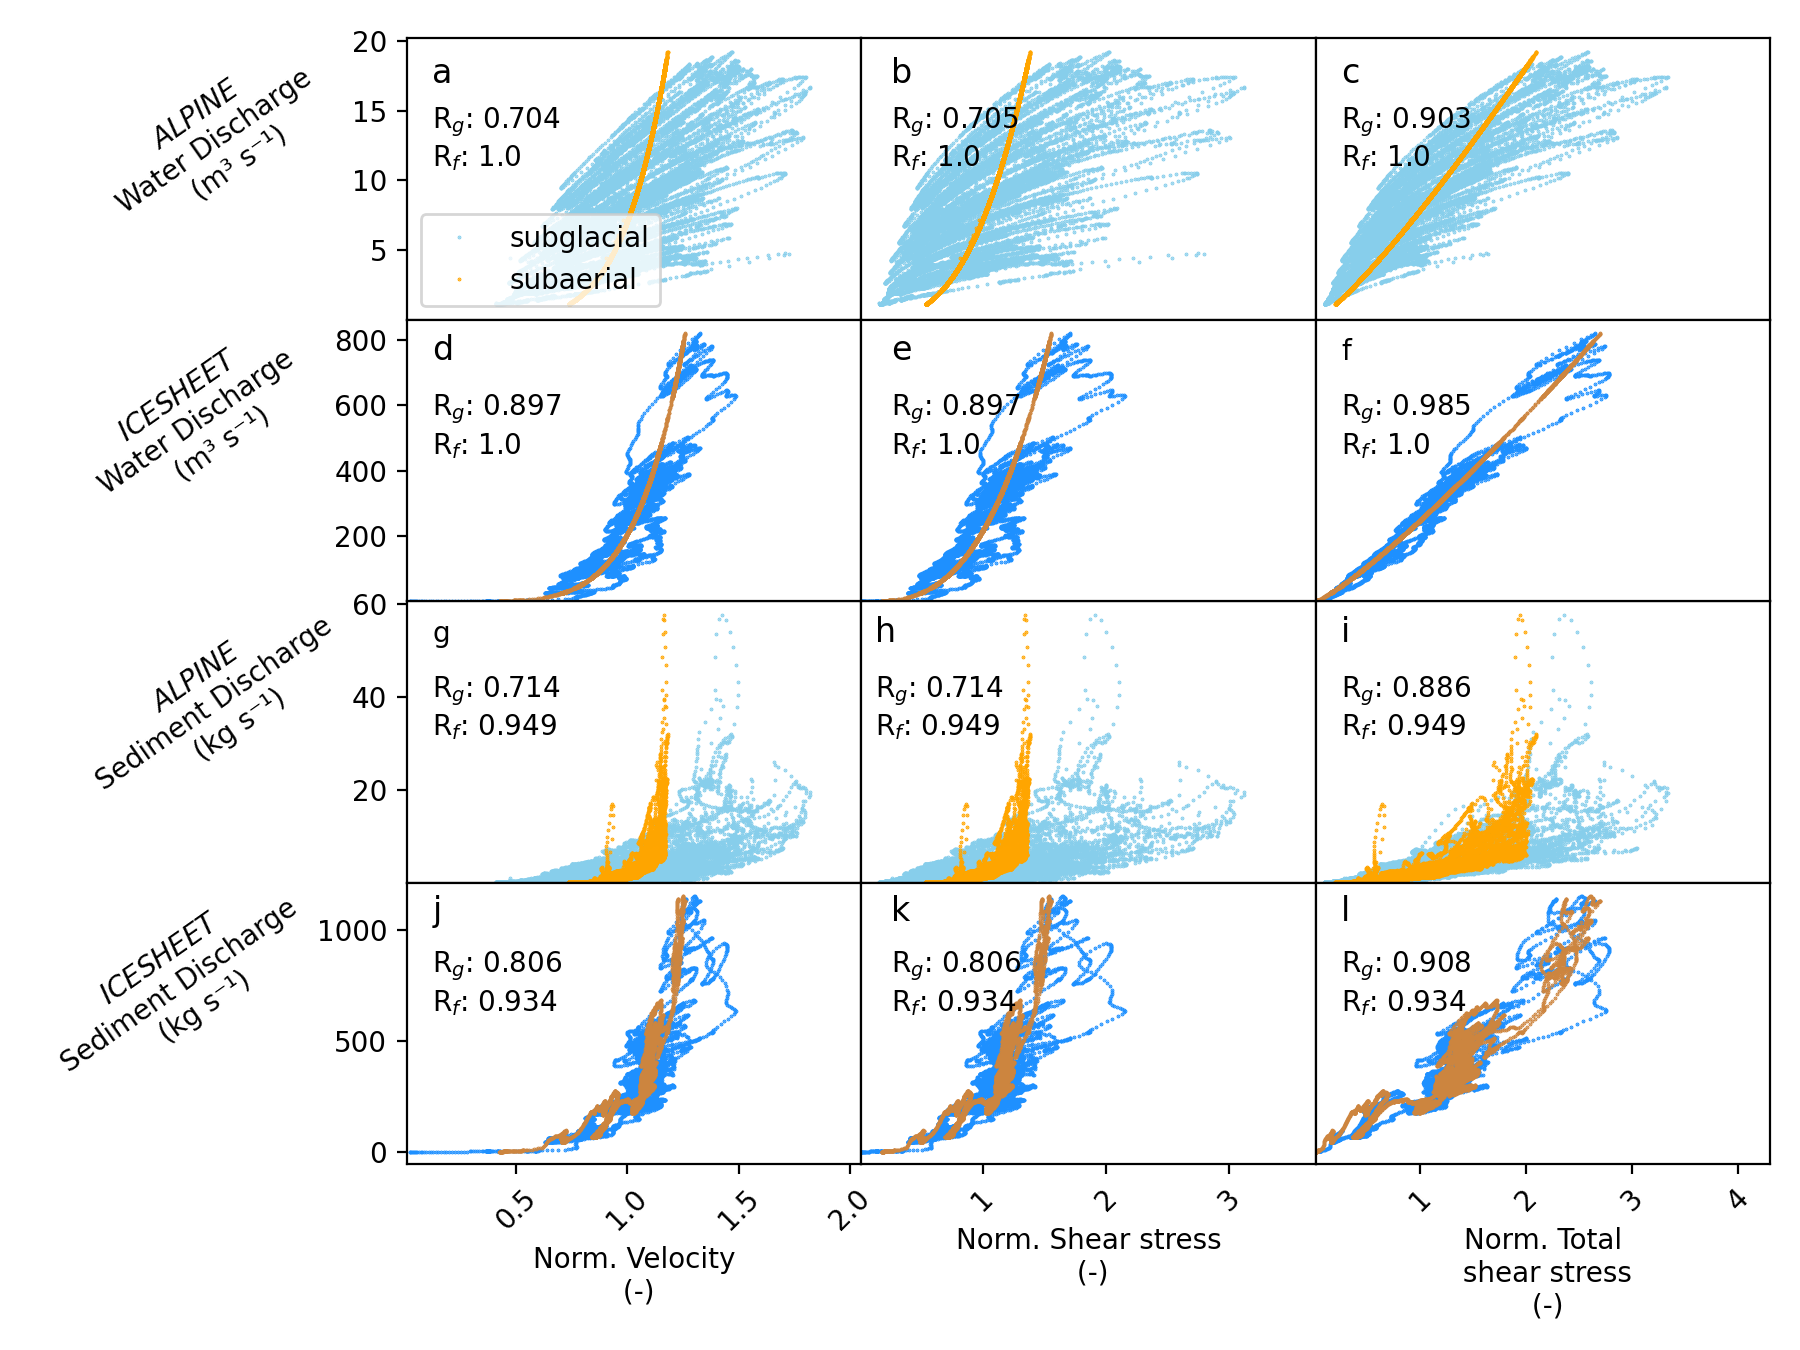
\includegraphics[width=0.7\linewidth]{Fig3_hr.png}
    \caption{As Figure \ref{fig:model_outs}, with $1$ \,\unit{hr} aggregation.} 
    \label{fig:model_outs_1hr}
  \end{figure}
\end{center}

\begin{center}
  \begin{figure}[h]
    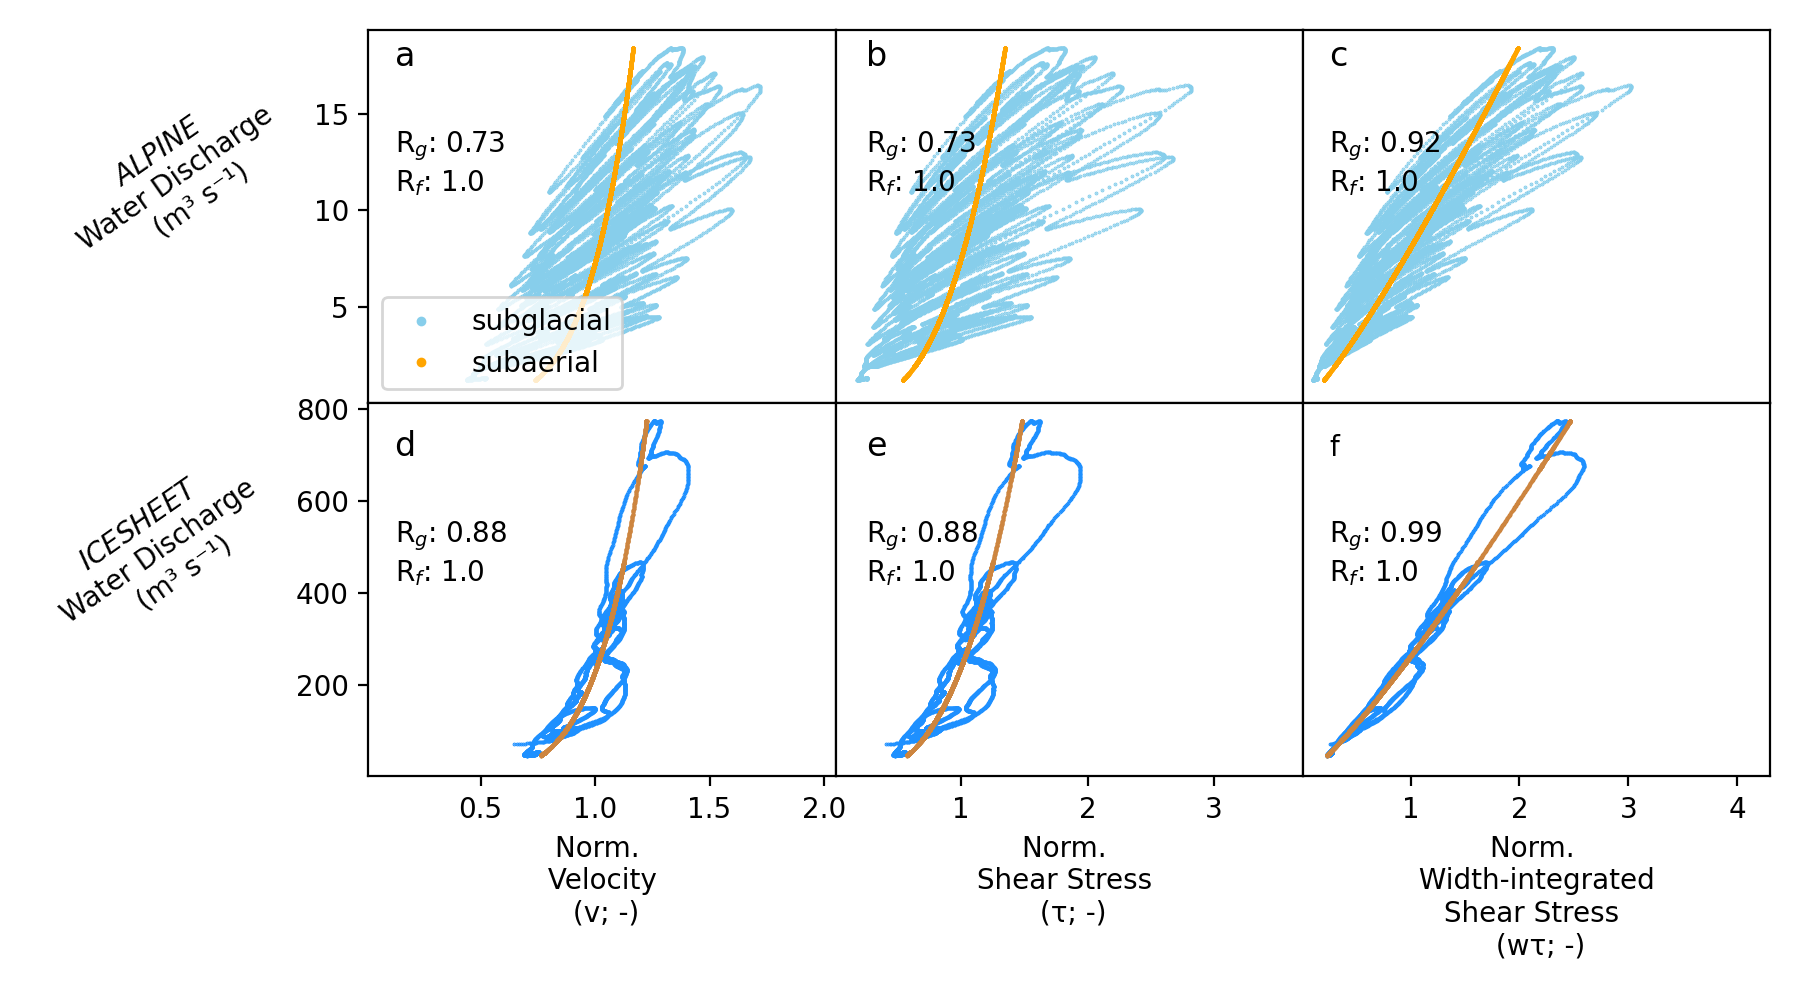
\includegraphics[width=0.7\linewidth]{Fig3_12hr.png}
    \caption{As Figure \ref{fig:model_outs}, with $12$ \,\unit{hr} aggregation.} 
    \label{fig:model_outs_12hr}
  \end{figure}
\end{center}


\begin{center}
  \begin{figure}[h]
    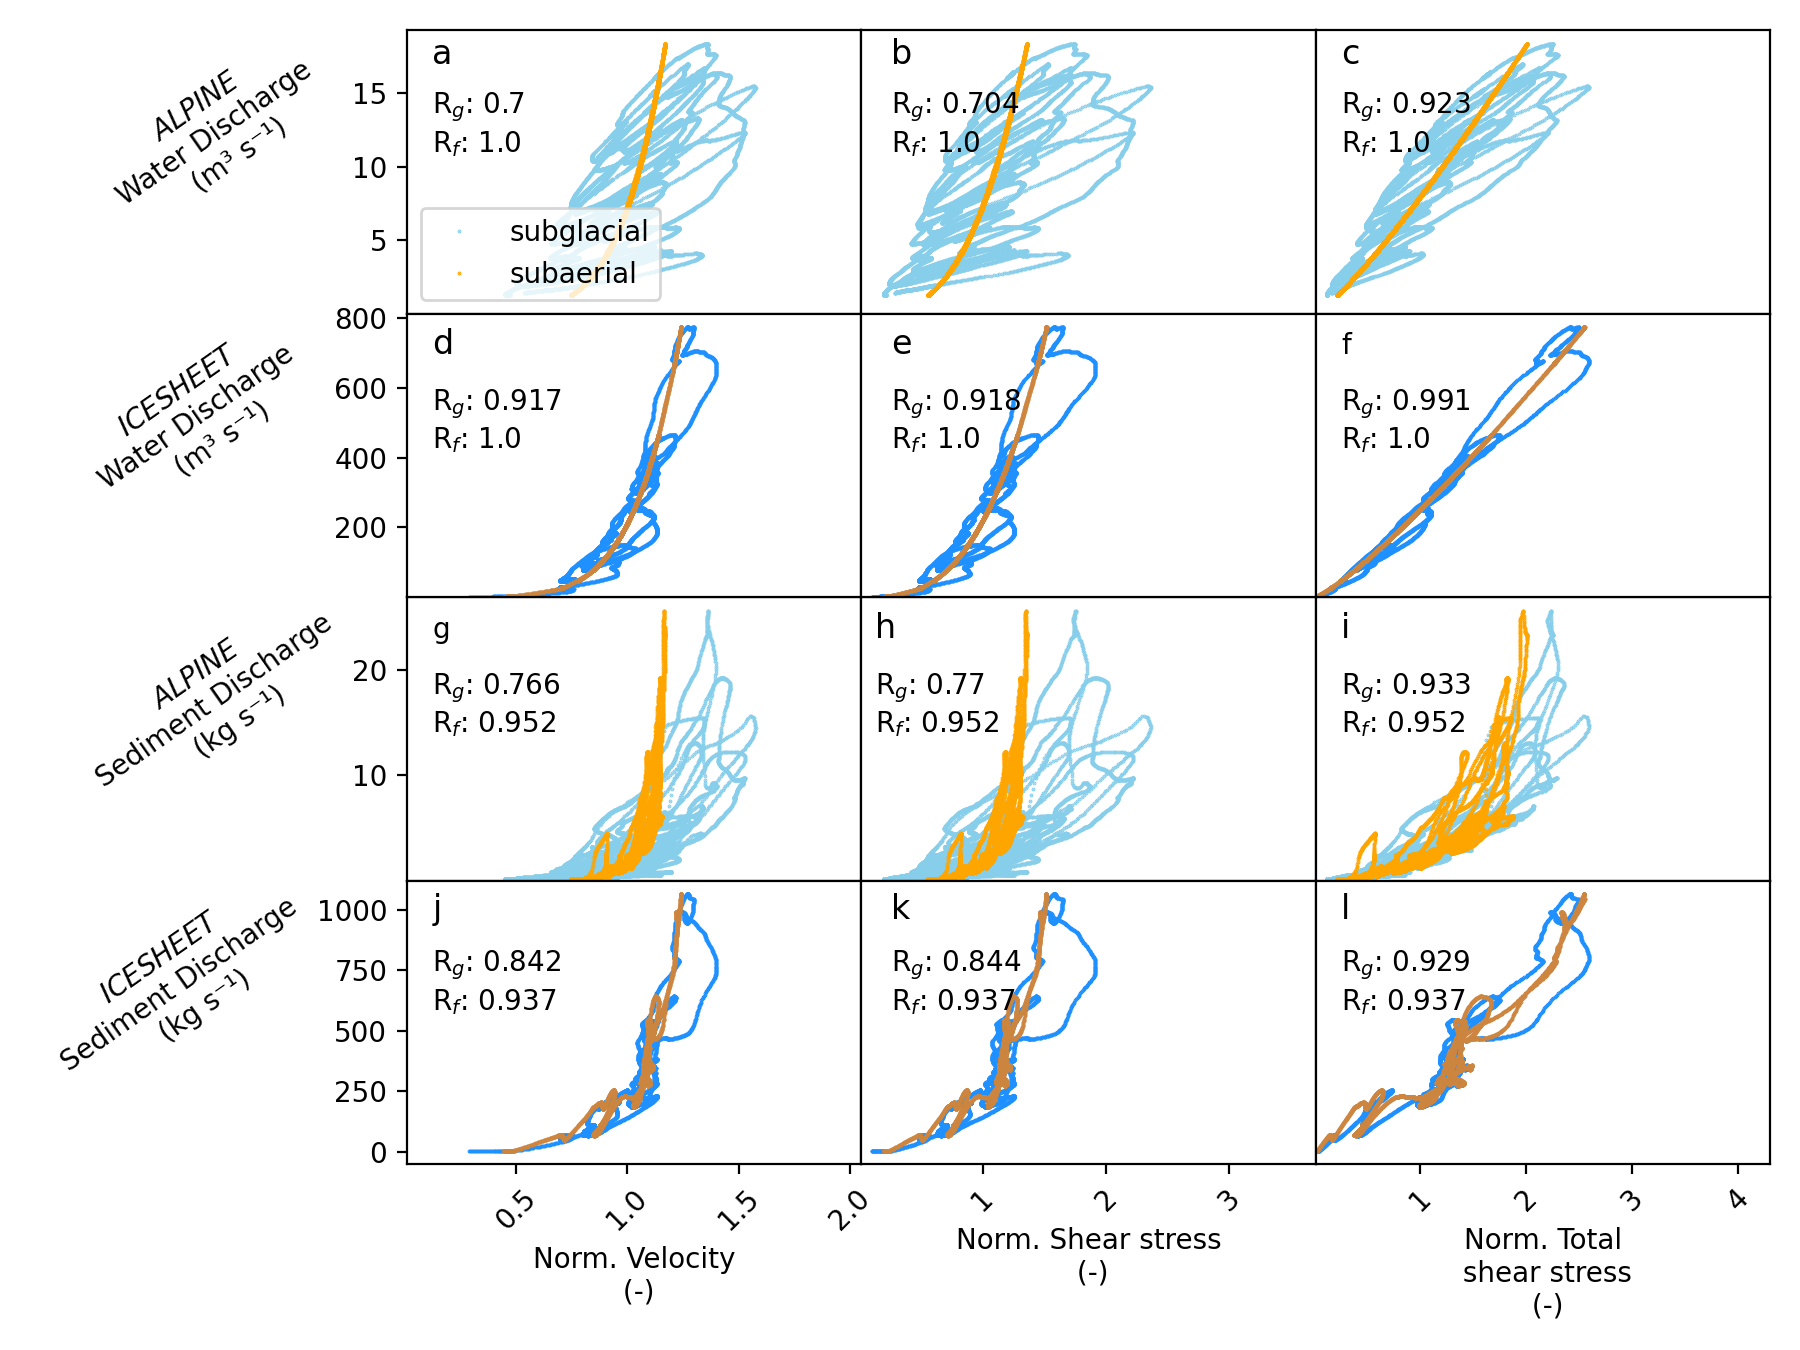
\includegraphics[width=0.7\linewidth]{Fig3_1day.png}
    \caption{As Figure \ref{fig:model_outs}, with $1$ \,\unit{day} aggregation.} 
    \label{fig:model_outs_1day}
  \end{figure}
\end{center}


\begin{center}
  \begin{figure}[h]
    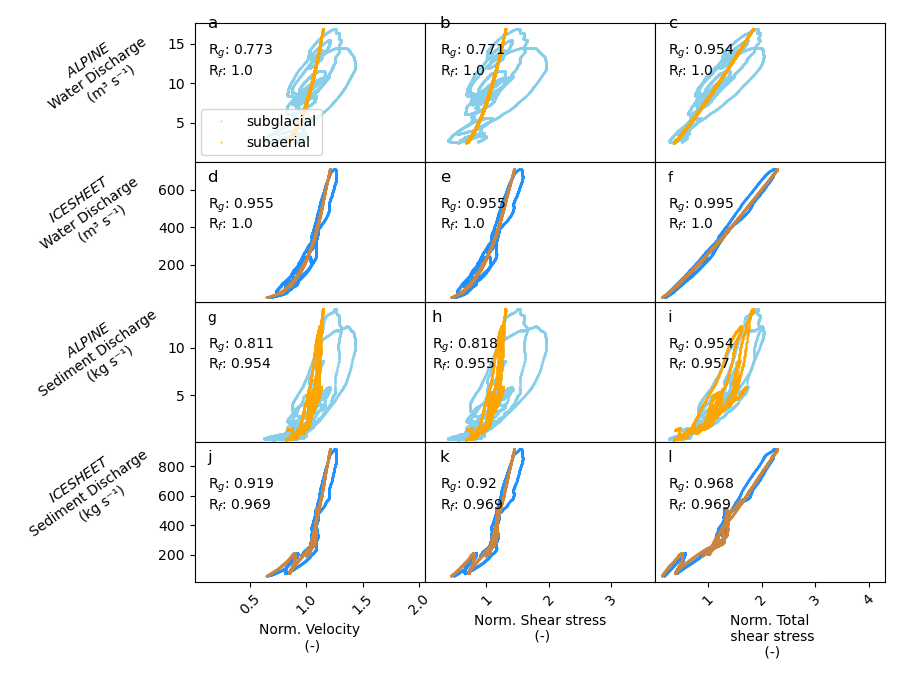
\includegraphics[width=0.7\linewidth]{Fig3_5day.png}
    \caption{As Figure \ref{fig:model_outs}, with $5$ \,\unit{day} aggregation.} 
    \label{fig:model_outs_5day}
  \end{figure}
\end{center}

\begin{center}
  \begin{figure}[h]
    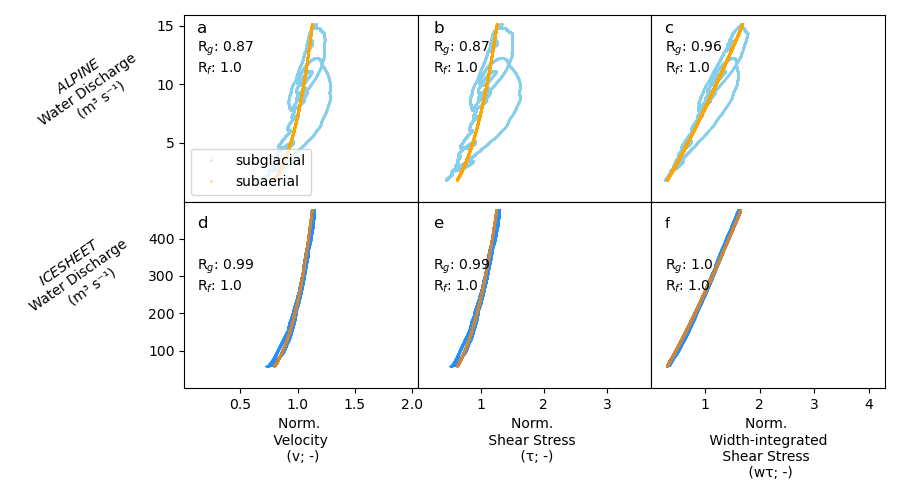
\includegraphics[width=0.7\linewidth]{Fig3_10day.png}
    \caption{As Figure \ref{fig:model_outs}, with $10$ \,\unit{day} aggregation.} 
    \label{fig:model_outs_10day}
  \end{figure}
\end{center}
\begin{center}
  \begin{figure}[h]
    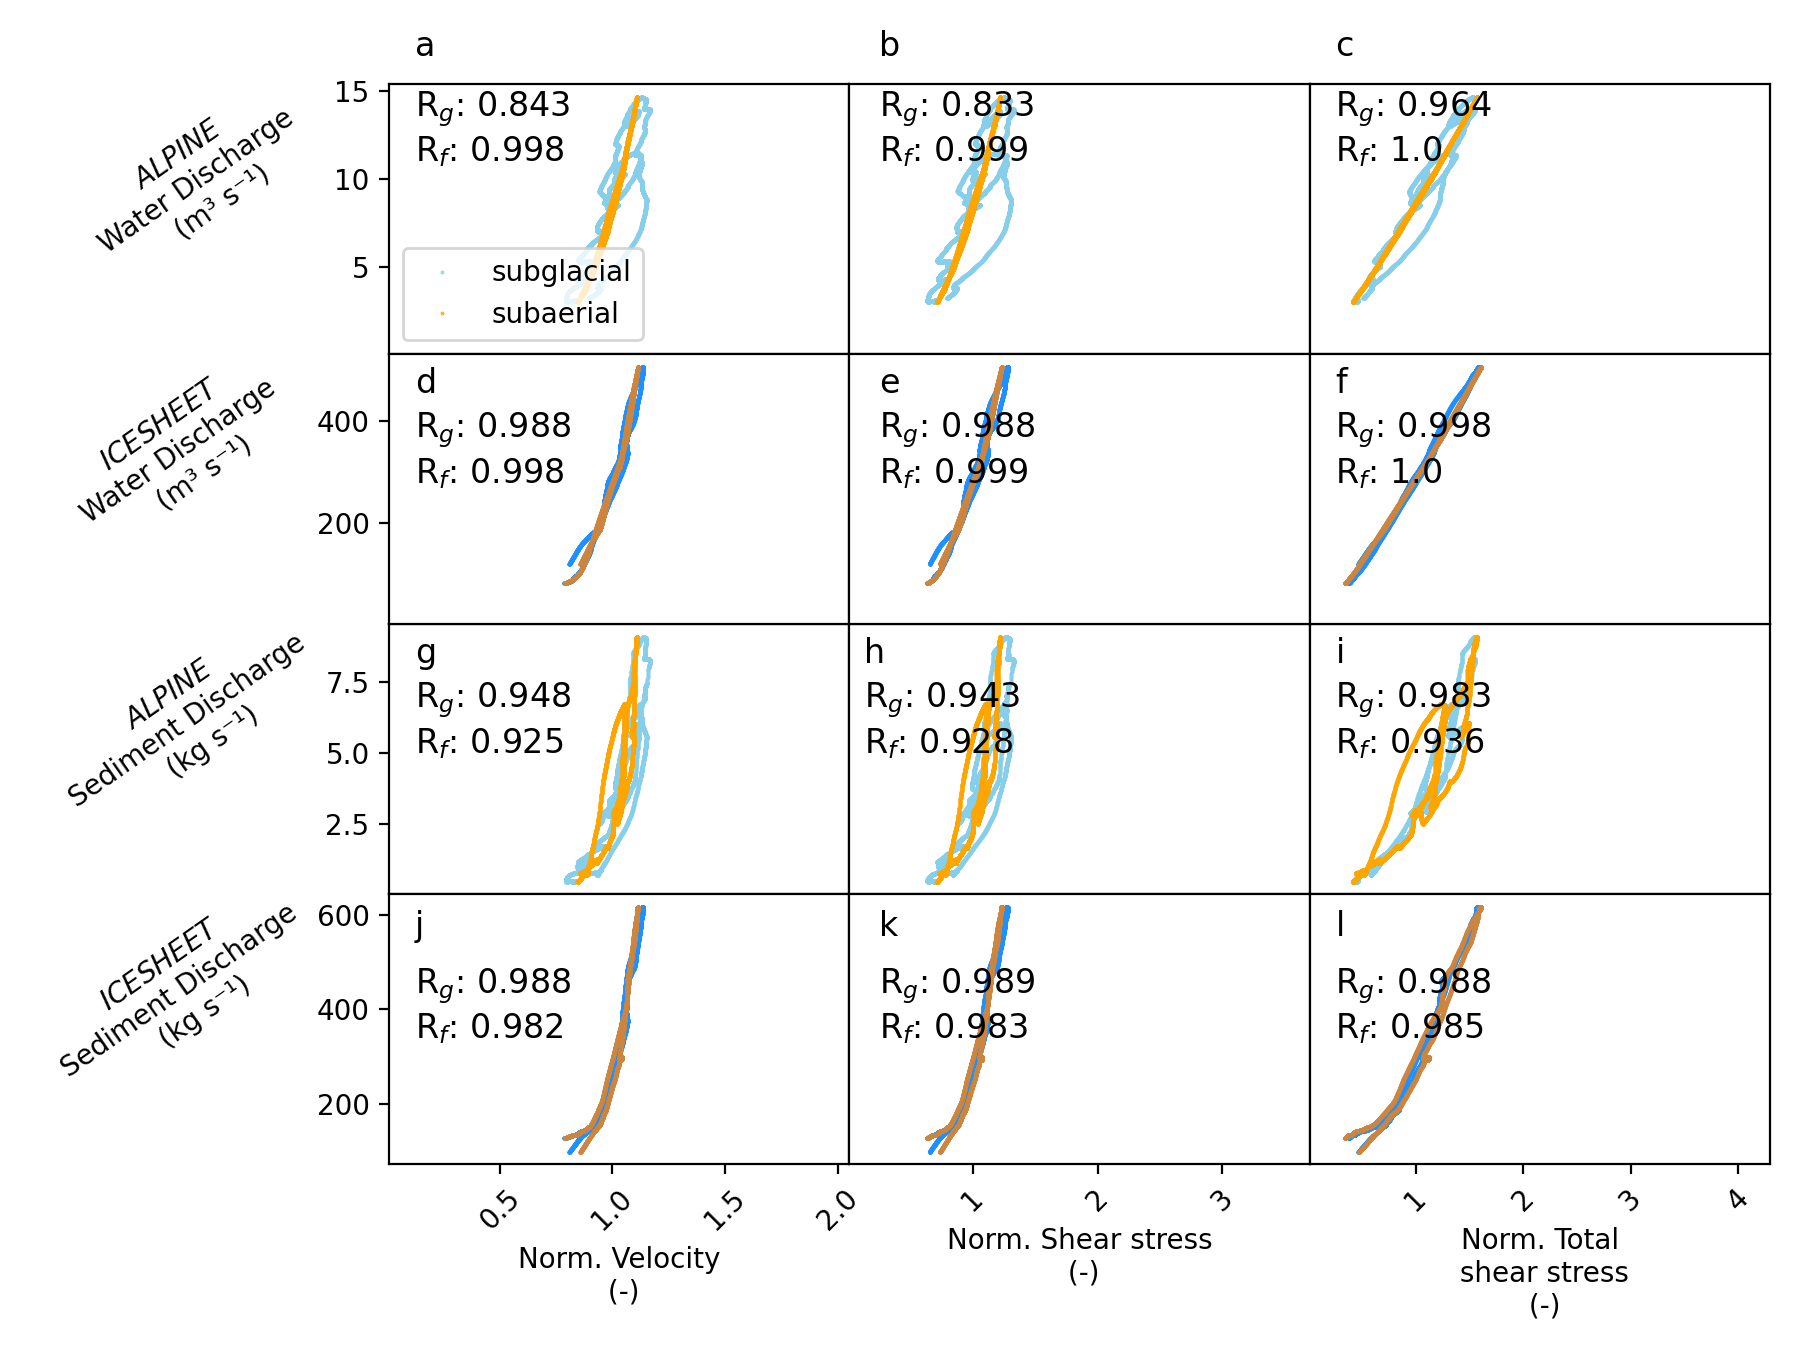
\includegraphics[width=0.7\linewidth]{Fig3_15day.png}
    \caption{As Figure \ref{fig:model_outs}, with $15$ \,\unit{day} aggregation.} 
    \label{fig:model_outs_15day}
  \end{figure}
\end{center}

\end{document}

These different characteristics between glacial and subaerial channels show that records of sediment transport downstream of glaciers represent both subglacial and subaerial processes together.
Divergent processes discussed here might be particularly relevant at glacier margins, where water transitions from pressurized subglacial flow to open-channel subaerial flow.
The inconsistent response of sediment transport in subglacial and subaerial systems to changing water discharge could add uncertainty in evaluating  sediment transport signals in subglacial systems.
In addition, the subglacial parameterization shows that sediment transport capacity in glacier systems responds to a large number of factors such as channel size, ice thickness, and glacier surface slope, which may react to climate forcing differently than water discharge alone.


In natural systems, variable mobilization and deposition of sediment occur as water and sediment discharge accumulate as they move through the two-dimensional channel network will compound the already substantial variability in sediment mobilization parameters accounted for here in the lumped parameterization.
Such variability could be especially strong in the subglacial system where meltwater pathways change in response to the evolving hydraulic gradient \citep{delaney2023}.


Results here suggest that increased variability in sediment transport in subglacial systems  could be particularly pronounced on ice sheets with large catchments and reduced water discharge variability over sub-monthly timescales.
Furthermore, width-integrated shear stress across the channel bed can remain relatively high across a range of water discharges (Figures~\ref{fig:model_outs} and \ref{fig:Qw_vari}).
\TODO{is this needed?... does if conflict with observations of the Leverett and not testable} 
